
\section{De Haas-van Alphen torque oscillation}

In this section the phenomenon of \ac{dHvA} oscillations is described along with its measurement by the torque method. For decades, \ac{dHvA} has provided the principle method of characterising the Fermiology of a material with only relatively recent competition from techniques such as positron annihilation and \ac{ARPES} in particular. Whilst \ac{ARPES} can provide direct maps of Fermi surfaces within the Brillouin zone, \ac{dHvA} has some advantages such as the fact that it ignores surface effects such as crystal reconstruction, can determine cross-sectional areas with a relatively high resolution and also provides useful secondary measurements such as effective masses of the quasiparticle carriers.  Some disadvantages of the technique include the fact that \ac{dHvA} cannot locate particular cross-sectional orbits within the Brillouin zone (thus relies on secondary knowledge such as \ac{DFT} calculations) and also that the high magnetic fields could potentially affect the Fermi surface, for example by splitting the energy levels. Regardless \ac{dHvA} continues to be a reliable technique for Fermi surface characterisation. A more detailed comparison of all three techniques can be found in appendix~\ref{Appendix:FermilogyTechniques}.



\subsection{Theory}

\subsubsection{Overview}

For metals, the majority of the interesting physics occurs at the Fermi level and, provided Fermi liquid theory holds true, the electrons at the Fermi level can be modelled to a high degree of accuracy with the Sommerfeld model --- that is a Fermi gas of non-interacting electrons in an infinite box. When a magnetic field is applied, the electrons have their usual grid pattern distribution of plane wave k-vectors rearranged such that the electrons move around orbital and helical paths. These rearranged k-vectors form a set of concentric tubes, known as Landau tubes, whose cross-sectional area, $a$, perpedicular to the field is given by the Onsager relation:\footnote{Derivations of the Onsager relation are given in several textbooks including pg. 32 of Schoenberg\cite{Schoenberg1984} and pg. 272 of Ashcroft \& Mermin\cite{Ashcroft1976}.} 
%%
\begin{equation}
\label{Eqn:2:Onsager}
\textit{a}_{k_{\perp}} = (r + 1/2)\frac{2\pi e B}{\hbar}
\end{equation}
%%
where $r$ is a quantisation number that sets apart each tube. We can see from the relation that as $\vect{B}$ increases, so does the cross-sectional area of the tubes. As the magnetic field is ramped, successive tubes periodically pass the Fermi surface causing a spike in the \ac{DOS} at the Fermi level and also oscillations in the energy o the ssytem, $E$, which, for geometric reasons explained in the next section, are far stronger at the maximumal and minimal (extremal) areas of Fermi surface. Thermodynamic quantities such as magnetic susceptibility ($\chi = \partial E/\partial B$) and heat capacity ($C_{V} = \partial^2E/\partial T^2|_{V}$) or quantities that depend on the \ac{DOS} at the Fermi level such as electrical resistance all oscillate as the field is ramped. Oscillations in the susceptibility are known as \ac{dHvA} oscillations, oscillations in the resistivity are known as Shubnikov-de Haas oscillations.

 We can relate the `frequency' $F$ (measured in $tesla$\footnote{n.b. that it is \textit{tesla} and not \textit{tesla$^{-1}$} because, as we shall see later, the oscillations are actually periodic in $1/B$ and \textit{not} $B$ so their frequency counterpart is measured in \textit{tesla}.}) that the tubes pass the Fermi surface to the extremal Fermi surface area using the following application of the Onsager relation,
%%
\begin{equation}
\textit{a}_{k_{\perp}} = \frac{2\pi e }{\hbar}F
\end{equation}
%%
By varying the direction of the field we can obtain a series of maximal and minimal Fermi surface areas in a variety of orientations in order to build a profile of the Fermi surface topology and size. In practice, there are many possible variations that might fit the model based on areas of cross-sectional slices alone and so typically ab-initio \ac{DFT} calculations --- described in section~\ref{Sec:2:dft} --- are employed to provide a basis which can be tweaked based on the constraints from the measurements. 

A more detailed analysis of this process follows, beginning with an illustrative mathematical treatment for oscillations in the magnetisation.

\subsubsection{Oscillations in magnetisation}

We begin by calculating the degeneracy of the Landau tubes i.e. the number of electron states per tube. Because the states under a magnetic field are a one-to-one rearrangement of the states with no field, we can use the Sommerfeld number of states per unit k-space ($V/4\pi^3$) to determine the degeneracy. From the Onsager relation (eqn.\ref{Eqn:2:Onsager}) we see that the additional area for successive tubes is $\Delta a_{k_{\perp}}  = 2\pi e B/\hbar$ which we can convert to a volume by integrating over $k_{\perp}$. This gives a degeneracy per tube therefore of,

\begin{equation}
D_{\textrm{tube}} = d k_{\perp}\left(\frac{2\pi e B}{\hbar}\right)\left(\frac{V}{4 \pi^3}\right) = \frac{eBVdk_{\perp}}{\hbar 2\pi^2}
\end{equation}

We continue by writing an expression for the energy of the system, $E$ by summing the energies of the states that lie beneath the cross-sectional area defined by the Fermi surface ($a_{k_\perp F}$) for a given $k_\perp$. To do this, we use the Onsager equation to determine $R_\perp$ --- the number of Landau tubes below the Fermi surface at this cross-sectional slice. We then multiply this by the degeneracy of the tubes, $D$ and the energy for states on that particular Landau tube, $\epsilon_r$,
%%
\begin{equation}
\label{Eqn:2:OscillateE}
E = D\sum_{r}^{R_\perp}\epsilon_r = \frac{eBVdk_\perp}{\hbar 2 \pi^2}\sum_{r}^{R_\perp}\epsilon_r
\end{equation}
 where,
\begin{equation}
R_\perp = \textrm{floor}\left[\frac{a_{k_\perp F}\hbar}{2\pi e B} - \frac{1}{2}\right]
\end{equation}
%%
To complete the above equation, we need an expression for the energies of each of the Landau tubes. The procedure for the free electron case is to insert the canonical momentum (i.e momentum of a free electron in a magnetic field) into the non-interacting Schr\"odinger equation and solve to obtain the following eigenvalues for the energies on the Landau tubes. Full derivations can be found in several textbooks\footnote{See for examples pg. 32ff. in Schoenberg\cite{Schoenberg1984} or pg. 148ff. in Blundell\cite{Blundell2001}.} and so will  not be repeated here. Below is the expression for the energy eigenvalues,
%%
\begin{equation}
\epsilon_r=(r+1/2) \hbar \omega_c + \frac{\hbar^2 k^2}{2m_0}
\end{equation}
%%
where,
%%
\begin{equation}
\omega_c = \frac{eB}{m_0}
\end{equation}
%%
and is known as the \textit{cyclotron frequency}. The summation term in equation\ref{Eqn:2:OscillateE} can now be written,
%%
\begin{align*}
\sum_r^{R_\perp}\epsilon_r &= \sum_r^{R_\perp}\left( (r+1/2) \hbar \omega_c + \frac{\hbar^2 k^2}{2m_0} \right) \\
    &= \frac{\hbar eB}{m_0}\sum_r^{R_\perp}r + \frac{\hbar eB}{2m_0}\sum_r^{R_\perp}1 + \frac{\hbar^2 k^2}{2m_0}\sum_r^{R_\perp}1 \\
    &= \frac{\hbar eB}{2 m_0} R_\perp(R_\perp + 1) + \frac{\hbar eB}{2m_0}R_\perp + \frac{\hbar^2 k^2}{2m_0}R_\perp \\
    &= \frac{\hbar eB}{2m_0}R_\perp^2 + \left(\frac{\hbar eB}{m_0} + \frac{\hbar^2 k^2}{2m_0}\right)R_\perp
\end{align*}
%%
which can be expanded out and finally substituted back into equation\ref{Eqn:2:OscillateE} to finally obtain,
%%
\begin{equation}
\label{Eqn:2:OscIllustration}
E = \frac{eB^2Vdk_\perp}{4\pi^2m_0}\left[e R_\perp^2 + \left(2e + \frac{\hbar k^2}{B}\right)R_\perp\right]
\end{equation}
%%
Key to the above relation is that, although $R_\perp$ is inversely proprtional to $B$, it remains discrete. This gives rise to the saw-tooth like function shown in \fig\ref{Fig:2:EnergyOscillations} for some typical experimental parameters. Also plotted is the fuction against $1/B$ where we can clearly see that the oscillations are periodic in inverse field hence the frequency being measured in tesla$^{-1}$.
%%
\begin{figure}[htbp]
    \begin{center}
        \includegraphics[scale=0.9]{Chapter2-ExperimentalTechnique/Figures/TheoreticalOscillations/TheoreticalOscillations}
        \caption{Theoretical energy oscillations for a Fermi surface orbit which is 5\% of a \unit[5]{\AA} cubic Brillouin zone between \unit[1--18]{T}. Kinetic energy term is taken to be for an electron at a level half the size of the Fermi surface.}
        \label{Fig:2:EnergyOscillations}
    \end{center}
\end{figure}

The above is not a rigourous derivation but is nonetheless illustrative of the origin of the oscillation in the system energy and how any thermodynamic value which depends on the energy of the system oscillates as a function of field. To continue we need to include correction factors to the oscillation amplitude due to finite electron scattering rates ($A_D$), temperature ($A_T$), Zeeman splitting of spins ($A_s$), doping ($A_{\textrm{dop}}$), mosaicity ($A_{\textrm{mos}}$), warping of the Fermi surface ($A_{\textrm{warp}}$) as well as adjustments due to the fact that the parameter measured was torque of the sample in a field and not the energy or magnetisation directly ($A_{\Gamma}$). For this, we turn to a more solid foundation that was put forward by Lifschitz and Kosevitch and presented by Schoenberg.

\subsubsection{\acl{LK} equation}

The derivation for the full expression for the Landau thermodynamic potential, $\Omega$\footnote{Formally defined as the energy in a open system that is in thermal contact with its surroundings}, begins in a similar way to the previous illustrative example but frames the sawtooth-like function above as a more mathematically manageable Fourier decomposition which also conveniently makes the technique highly amenable to Fourier analysis. For this reason the equation below features higher harmonics which are denoted with the identifier $p$.
%%
\begin{equation}
\Omega = \left(\frac{e}{2\pi\hbar}\right)^{\frac{3}{2}}\frac{e\hbar B^{\frac{5}{2}}}{m_0 \pi^2}\left| \frac{\partial^2 a_{\textrm{ext}}}{\partial k^2_\perp}\right|^{-\frac{1}{2}}\sum_{p=1}^{\infty}p^{-\frac{5}{2}}A\cos\left[2\pi\left(\frac{F}{B} - \gamma\right)\pm\frac{\pi}{4}\right]
\end{equation}
where,
\begin{equation}
A = A_T A_D A_s A_{\textrm{mos}} A_{\textrm{dop}} A_{\textrm{warp}} 
\end{equation}
The above equation and derivatives of it are known as the \ac{LK} equation. We no longer have the integral over $k_\perp$ and instead have the parameter $a_{\textrm{ext}}$ which is (one of) the extremal Fermi surface orbit area(s) perpendicular to a particular field direction. Only the extremal (i.e. the largest and smallest) magnetically induced orbits contribute significantly to oscillations in the system energy. The reason for this is that when performing the integral over $k_\perp$ to attain the \ac{LK} equation, $F$ varies as a function of $a_{k_\perp}$ and hence as a function of $k_\perp$. This leads to a blurring of the phase in the cosine term for a given $B$ which reduces the overall amplitude significantly. Regions where $dF/dk_\perp$ is small (i.e. turning points) therefore have more orbits across the integration that are closely in phase and are therfore stronger

TODO

The modifications to the \ac{LK} equation listed towards the end of the previous section can be manifest by convolving an appropriate phase distribution function with the cosine oscillatory term. It can be shown\footnote{See for example, Schoenberg pg 57--59.\cite{Schoenberg1984}} that this convolution results in a relatively simple multiplication factor, hence the various $A$ factors listed in the equation.


\subsubsection{Extracting the effective mass from the temperature}

The temperature effects on the \ac{LK} equation are One possible way to introduce temperature effects is to consider that the Fermi energy $\mu$ may be smeared according to the Fermi distribution $f(\epsilon) = 1/(1+\exp((\epsilon-\mu)/kT))$.





Originally \ac{dHvA} measurements were used to measure the Fermi surfaces of elemental metals and so the initial assumption of a free-electron gas is justified based on the fact that elemental metals have a Fermi surface and are considered materials that adhere to Fermi liquid theory. The fact that oscillations have been observed in cuprates and pnictides which have demonstrated non-Fermi liquid behaviour is therefore remarkable and moreover implies the presence of a Fermi surface, at least in the prescence of a strong magnetic field.



\subsection{Mapping the Fermi surface}

\subsubsection{Background removal}
% TODO: Removal of background should not be done against 1/B as a rule.
% Include investigation as to low frequency peak
Previous standard practice was to remove a background polynomial fitted to the field or inverse field from the raw data before taking the FFT. \Fig\ref{Fig:2:BackgroundSubtraction} shows raw torque data taken over a range of angles\footnote{See section\ref{Sec:3:AngleDependentMeasurements} for full details} and a strong $H^2$ component can be observed as a result of the $R_{\Gamma}$ term in equation\ref{}. Subtracting a second order polynomial fitted to the \textit{inverse} field leaves a large artificial angle-dependant oscillation in $1/H$ in the residual which may be misconstrued as a signal from a low frequency Fermi surface orbit. For this reason it is recommended to subtract a second order polynomial fitted to field rather than inverse field for torque measurements.
\begin{figure}[h!]
    \begin{center}
        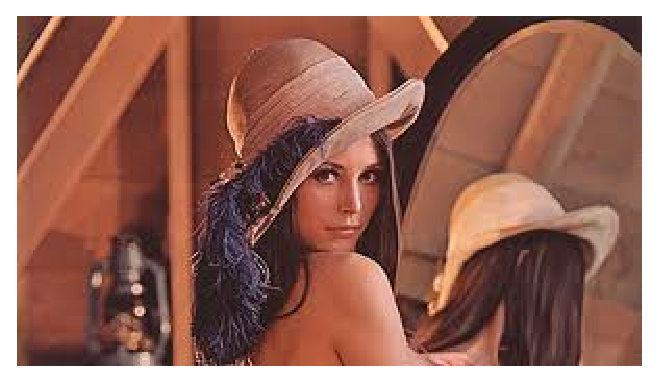
\includegraphics[scale=0.7]{Misc/TODO}
        \caption{Left panel shows the angle dependance of the raw torque signal  clearly showing a positive $H^2$ component for $\theta>0$ and a $-H^2$ component for $\theta<0$. Centre panel shows the FFT vs. angle for data with the 2nd order polynomial fitted to $1/H$ removed. A strong angle dependant peak at low frequency is seen. Right panel shows the same data but with a second order polynomial fitted to $H$ removed.}
        \label{Fig:2:BackgroundSubstraction}
    \end{center}
\end{figure}



\subsection{Measuring the spin mass}

\subsection{Measuring the band mass}

\subsubsection{Basic LK formula fitting}

Of all the damping terms in the \LK equation, only $R_T$ has any kind of temperature dependancy. This term also features the effective mass. By measuring oscillations at a fixed angle but with varying temperatures, the effective mass can be determined. However there is a difficulty in that in-order to observe oscillations, it is necessary to sweep the magnetic field, and many other damping terms have a field dependancy. To the first approximation, an inversely averaged applied field can be used in the \LK equation provided that the field sweep range is small. However there are a couple of techniques that were employed in order to overcome this shortcoming.

\subsubsection{Retrofitting ansatz LK formulae}
\label{Sec:2:LKRetrofitting}

One of the primary field-dependant contributions to the oscillation amplitude is the Dingle term scattering (equation \ref{Eqn:2:DingleTermOscillationAmp}). This has an exponential dependance with temperature. The Dingle factor, $\alpha$, can be determined by fitting a simplified version of equation \ref{Eqn:2:OscillationAmp} to oscillations which have been filtered to reduce the number of fitting parameters. Once we have the Dingle term, a series of ansatz data TODO...




\subsubsection{`Microfitting' the LK formula}
\label{Sec:2:LKMicrofitting}

\subsection{Method}

Two separate arcs of extremal area were mapped for the angle dependent measurements. One goes along the arc from $B\parallel c$ towards the $a$ axis, the other goes along the arc from $B\parallel c$ towards the $110$ direction. The former we call the $100$ arc, the latter the $110$ arc. In fact, measurements start further back beyond the $B\parallel c$ direction in order to ensure that the minima was reached and to correctly align the crystal as described below.

\subsubsection{Angle correction}
    \label{Sec:2:AngleCorrection}

To perform angle dependent measurements, we need to first of all measure accurately the angle between subsequent measurements and second we need to determine the angle of the field compared to the basel planes of the crystal. A further problem is that of aligning the basel plane with respect to the arc of rotation, something that is discussed, briefly here, but in more detail in the results in section~\ref{Sec:3:DFTShifts}.

In order to tackle the first problem, the sample platform is subject to a weak oscillating magnetic field from a large coil mounted inside of the yellow cryostat.\footnote{An upper bound on the strength is $\sim$\unit[500]{Gauss}, based on \unit[2.2]{mV} after $\times100$ amplification measured across a coil of $\sim140$ turns with an average area of \unit[3.36]{$mm^2$} per loop} A voltage is induced in a smaller coil which is mounted on the rotating portion of the sample platform\footnote{In fact there are two small coils, each perpendicular to one another although only one is measured at a time} which is proportional to the sine of the angle between the coil and the AC field. By monitoring this voltage, accurate determination of the angle between the sample platform and the field can be made and therefore the angle between subsequent measurements.

The correct angle between the large DC field and the crystal planes in the sample were determined using a post-measurement correction. Since the frequency of the quantum oscillations are field dependent with turning points at the $H\parallel [001]$ direction for approximately two dimensional samples, an even termed polynomial up to fourth order was fitted to the peaks. From the minima of the fits an angular offset was obtained which gave the final correction to the above coil measurements.

The basel angle was aligned on the cantilever by eye. This was coupled with XRD measurements which determined how the visual features corresponded to the crystal axes. This leads to an estimated error in basel plane alignment of around \unit[5]{\%} although we found evidence for greater misalignment in one case, detailed in the results.

\subsubsection{Temperature correction}
    \label{Sec:2:TemepratureCorrection}

Effective mass measurements on particular extremal orbits rely on accurate temperature determination at all stages of the field sweep. On the Yellow magnet system, temperature from base of $\approx$\unit[0.3]{K} to $\approx$\unit[2]{K} is controlled by adjusting the He$^3$ sorbtion pump temperature and can be considered to be independant of field effect since the thermometer regulating the sorb temperature is outside of the strong field core. However if we consider \fig\ref{Fig:2:TemperatureCorrection}, it is evident that there are magnetic field effects on the RuOx, which is mounted in the base of the magnet but thermally linked with the sample, and the Cernox thermometer that sits on the sample stage.
\begin{figure}[htbp]
    \begin{center}
        \includegraphics[scale=0.9]{Chapter3-dHvABaFe2P2/Figures/Mass/TemperatureCorrection/TemperatureCorrection}
        \caption{Some example temperature readings (squares) set using the sorbtion pump heater. Also shown are corrections (circles) by interpolating to known values. RuOx thermometer is shown in blue, Cernox stage thermometer is shown in red. Second order polynomial fits to the data are shown as lines extrapolated to zero to get a rough estimate of the zero field temperature value.}
        \label{Fig:2:TemperatureCorrection}
    \end{center}
\end{figure}
Readings from both thermometers were taken with field sweeps from zero field up to \unit[18]{T} at steady temperatures \unit[0.30]{K}, \unit[0.53]{K}, \unit[0.64]{K}, \unit[1.06]{K} and \unit[1.34]{K}. By interpolating between this data\footnote{Performed using multiquadric radial basis functions from the Scipy Python library.}, the two thermometers can be correctied to agree within $\sim$\unit[0.01]{K}. This interpolation is however limited to temepratures below approximately \unit[1.45]{K} as is shown in the figure for readings at around \unit[1.6]{K}. In these cases, the less reliable method of extrapolating the readings back to zero field using a second order polynomial fit are used as demonstrated with the solid lines in \fig\ref{Fig:2:TemperatureCorrection}. In these cases the temeprature is taken to be the mean of the two extrapolated values with the differences defining the error.


\subsection{Yellow Magnet}

dHvA Measurements were all performed in Bristol on the `Yellow Magnet' system which was built by Oxford and can nominally operate up to \unit[20]{t} with use of the lambda plate although more typically is operated up to \unit[18]{T}. The sample sites on a one axis rotator and angle is determined by one of two orthogonal pick-up coils mounted on the sample stage weak, oscillating magnetic, field in

